\documentclass[xcolor={dvipsnames}]{beamer}
%\usepackage[utf8]{inputenc}
\usetheme{Madrid}
%\usetheme{Malmoe}
\usecolortheme{beaver}
%\usecolortheme{rose}

%-------------------------------------------------------------------------------
%          -Packages nécessaires pour écrire en Français et en UTF8-
%-------------------------------------------------------------------------------
\usepackage[utf8]{inputenc}
\usepackage[frenchb]{babel}
\usepackage[T1]{fontenc}
\usepackage{lmodern}
\usepackage{textcomp}

%-------------------------------------------------------------------------------

%-------------------------------------------------------------------------------
%                          -Outils de mise en forme-
%-------------------------------------------------------------------------------
\usepackage{hyperref}
\hypersetup{pdfstartview=XYZ}
\usepackage{enumerate}
\usepackage{graphicx}
%\usepackage{multicol}
%\usepackage{tabularx}

%\usepackage{anysize} %%pour pouvoir mettre les marges qu'on veut
%\marginsize{2.5cm}{2.5cm}{2.5cm}{2.5cm}

\usepackage{indentfirst} %%pour que les premier paragraphes soient aussi indentés
\usepackage{verbatim}
%\usepackage[table]{xcolor}  
%\usepackage{multirow}
\usepackage{ulem}
%-------------------------------------------------------------------------------


%-------------------------------------------------------------------------------
%                  -Nécessaires pour écrire des mathématiques-
%-------------------------------------------------------------------------------
\usepackage{amsfonts}
\usepackage{amssymb}
\usepackage{amsmath}
\usepackage{amsthm}
\usepackage{tikz}
\usepackage{xlop}
\usepackage[output-decimal-marker={,}]{siunitx}
%-------------------------------------------------------------------------------


%-------------------------------------------------------------------------------
%                    - Mise en forme 
%-------------------------------------------------------------------------------

\newcommand{\bu}[1]{\underline{\textbf{#1}}}


\usepackage{ifthen}


\newcommand{\ifTrue}[2]{\ifthenelse{\equal{#1}{true}}{#2}{$\qquad \qquad$}}

\newcommand{\kword}[1]{\textcolor{red}{\underline{#1}}}


%-------------------------------------------------------------------------------



%-------------------------------------------------------------------------------
%                    - Racourcis d'écriture -
%-------------------------------------------------------------------------------

% Angles orientés (couples de vecteurs)
\newcommand{\aopp}[2]{(\vec{#1}, \vec{#2})} %Les deuc vecteurs sont positifs
\newcommand{\aopn}[2]{(\vec{#1}, -\vec{#2})} %Le second vecteur est négatif
\newcommand{\aonp}[2]{(-\vec{#1}, \vec{#2})} %Le premier vecteur est négatif
\newcommand{\aonn}[2]{(-\vec{#1}, -\vec{#2})} %Les deux vecteurs sont négatifs

%Ensembles mathématiques
\newcommand{\naturels}{\mathbb{N}} %Nombres naturels
\newcommand{\relatifs}{\mathbb{Z}} %Nombres relatifs
\newcommand{\rationnels}{\mathbb{Q}} %Nombres rationnels
\newcommand{\reels}{\mathbb{R}} %Nombres réels
\newcommand{\complexes}{\mathbb{C}} %Nombres complexes


%Intégration des parenthèses aux cosinus
\newcommand{\cosP}[1]{\cos\left(#1\right)}
\newcommand{\sinP}[1]{\sin\left(#1\right)}

%Fractions
\newcommand{\myfrac}[2]{{\LARGE $\frac{#1}{#2}$}}

%Vocabulaire courrant
\newcommand{\cad}{c'est-à-dire}

%Droites
\newcommand{\dte}[1]{droite $(#1)$}
\newcommand{\fig}[1]{figure $#1$}
\newcommand{\sym}{symétrique}
\newcommand{\syms}{symétriques}
\newcommand{\asym}{axe de symétrie}
\newcommand{\asyms}{axes de symétrie}
\newcommand{\seg}[1]{$[#1]$}
\newcommand{\monAngle}[1]{$\widehat{#1}$}
\newcommand{\bissec}{bissectrice}
\newcommand{\mediat}{médiatrice}
\newcommand{\ddte}[1]{$[#1)$}

%Figures
\newcommand{\para}{parallélogramme}
\newcommand{\paras}{parallélogrammes}
\newcommand{\myquad}{quadrilatère}
\newcommand{\myquads}{quadrilatères}
\newcommand{\co}{côtés opposés}
\newcommand{\diag}{diagonale}
\newcommand{\diags}{diagonales}
\newcommand{\supp}{supplémentaires}
\newcommand{\car}{carré}
\newcommand{\cars}{carrés}
\newcommand{\rect}{rectangle}
\newcommand{\rects}{rectangles}
\newcommand{\los}{losange}
\newcommand{\loss}{losanges}


%----------------------------------------------------


\usepackage{../../../../pas-math}
\usepackage{../../../../moncours_beamer}

\usepackage{amssymb,amsmath}


\newcommand{\myitem}{\item[\textbullet]}

\graphicspath{{../img/}}

\title{Séquence 5 : Division}
\date{ }
%\author{O. FINOT}\institute{Collège S$^t$ Bernard}

%
\AtBeginSection[]
{
	\begin{frame}
		\frametitle{}
		\tableofcontents[currentsection, hideallsubsections]
	\end{frame} 

}
%
%
\AtBeginSubsection[]
{
	\begin{frame}
		\frametitle{Sommaire}
		\tableofcontents[currentsection, currentsubsection]
	\end{frame} 
}

\begin{document}



\begin{frame}
  \titlepage 
\end{frame}


\begin{frame}{}
	\begin{myobj}
	\begin{itemize}
		\item Je connais et j'utilise le vocabulaire des divisions;
		\item Je sais si un nombre est divisible par un autre ;
		\item Je sais poser et calculer la division d’un nombre entier par un autre ;
		\item Je sais  poser et calculer la division d’un nombre décimal par un nombre entier ;
		\item Je sais résoudre des problèmes en utilisant des additions, soustractions, multiplications et divisions.
		
	\end{itemize}
\end{myobj}

\begin{mycomp}
	\begin{itemize}
		%\begin{multicols}{2}
			
			
			\item \kw{Calculer } %: calculer avec des nombres rationnels, de manière exacte ou approchée, en combinant de façon appropriée le calcul mental, le calcul posé et le calcul instrumenté (calculatrice ou logiciel) ; 
			%\item \kw{Calculer (Ca2) } : contrôler la vraisemblance de ses résultats, notamment en estimant des ordres de grandeur ou en utilisant des encadrements ;
			\item \kw{Modéliser } %: traduire en langage mathématique une situation réelle (par exemple à l'aide d'équations, de fonctions, de configurations géométriques, d'outils statistiques) 
			\item \kw{Raisonner } 
			\item \kw{Représenter}
			\item \kw{Communiquer}
		%\end{multicols}
	\end{itemize}
\end{mycomp}
\end{frame}

\section{Division euclidienne}

\begin{frame}
	\begin{mydef}
		Effectuer la \kword{division euclidienne} d’un nombre entier, appelé \pause  \kword{dividende}, par un nombre entier, différent de zéro, appelé \pause  \kword{diviseur}, c’est trouver deux autres nombres entiers, le \pause \kword{quotient} et le \kword{reste}, tels que : \pause
		
		\begin{equation*}
			diviseur \times quotient + reste = dividende \pause	
		\end{equation*}
	\end{mydef}

	\begin{center}
		$\begin{array}{c|c}
			 & \hspace*{2cm} \\
			\cline{2-2}
			&  \\
			 & \\
		\end{array}$
	\end{center}

\end{frame}


\begin{frame}
	\begin{mydef}
		Effectuer la \kword{division euclidienne} d’un nombre entier, appelé   \kword{dividende}, par un nombre entier, différent de zéro, appelé   \kword{diviseur}, c’est trouver deux autres nombres entiers, le  \kword{quotient} et le \kword{reste}, tels que : 
		
		\begin{equation*}
			diviseur \times quotient + reste = dividende 
		\end{equation*}
	\end{mydef}
	
	\begin{center}
		$\begin{array}{c|c}
			Dividende & Diviseur \\
			\cline{2-2}
			& Quotient \\
			Reste & \\
		\end{array}$
	\end{center}
	
\end{frame}

\section{Multiples et diviseurs}

\subsection{Définition}

\begin{frame}
	\begin{mydefs}
	
			Quand le reste de la division euclidienne du nombre $a$ par le nombre $b$, différent de zéro, est égal à zéro, on dit que : \pause
			
			\begin{itemize}
				\item $a$ est \pause \kword{divisible} par $b$; \pause
				\item $a$ est \pause un \kword{multiple} de $b$; \pause
				\item $b$ est \pause un \kword{diviseur} de $a$. \pause
			\end{itemize}
		
	\end{mydefs}

\begin{myex}
	
	\begin{center}
		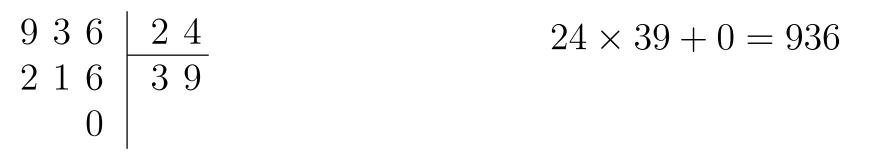
\includegraphics[scale=0.3]{../img/div} \pause
	\end{center}
	
	
	936 est divisible par 24 ; 936 est un multiple de 24 ; 24 est un diviseur de 936.\pause
\end{myex}

\begin{myexo}
	\begin{itemize}
		\item Citer 3 multiples de 24 :
		\item Citer tous les diviseurs de 16 :
	\end{itemize}
\end{myexo}

\end{frame}

\subsection{Critères de divisibilité}

\begin{frame}
	\begin{myprops}
		
		
			\begin{itemize}
				\item Un nombre entier est divisible par 2 si \pause \kword{il est pair} (son chiffre des unités est , 2, 4, 6 ou 8); \pause
				\item Un nombre entier est divisible par 5 si \pause son \kword{chiffre des unités est 0 ou 5}; \pause
				\item Un nombre entier est divisible par 10 si \pause son \kword{chiffre des unités est 0};	\pause
				
				\item Un nombre entier est divisible par 3 \pause si \kword{la somme de ses chiffres est divisible par 3}; \pause
				\item Un nombre entier est divisible par 9 si \pause \kword{la somme de ses chiffres est divisible par 9}; \pause
				
				\item Un nombre entier est divisible par 4 si \pause \kword{le nombre formé par ses chiffres des dizaines et ses unités} 
				
				\kword{ est divisible par 4}.
			\end{itemize}
		
	\end{myprops}
\end{frame}

\begin{frame}
	\begin{myexs}
		
			\begin{itemize}
				\item $1250$ est divisible par : \pause 2; 5 et 10. \pause 
				\item $726$ est divisible par : \pause 2 et 3. \pause
				\item $1024$ est divisible par : \pause 2 et 4.\pause
				\item $342$ est divisible par : \pause 2; 3 et 9.
				
			\end{itemize}
	
	\end{myexs}
\end{frame}

\end{document}